\section{Comparisons}
Now that we have the ability to do a $\DTCWT$ based scatternet, how does this
compare with the original matlab implementation \cite{oyallon_deep_2015} and the newly developed
KyMatIO \cite{andreux_kymatio:_2018}? \autoref{tab:ch3:scat_props} lists the different properties and 
options of the competing packages. 

\begin{table}
  \centering
  \mycaption{Comparison of properties of different ScatterNet packages}{In
  particular the wavelet backend used, the number of orientations available,
  the available boundary extension methods, whether it has GPU support and
  whether it supports backpropagation.}
  {\renewcommand{\arraystretch}{1.2}
  \begin{tabular}{@{}llllll}
    \toprule
    Package & Backend & Orientations & Boundary Ext. & GPU & Backprop \\\midrule
    ScatNetLight\cite{oyallon_deep_2015} & {FFT-based} & Flexible & Periodic & No & No \\
    KyMatIO\cite{andreux_kymatio:_2018} & {FFT-based}& Flexible & Periodic & Yes & Yes \\
    $\DTCWT$ Scat & {Separable filter banks} & 6 & Flexible & Yes & Yes \\
    \bottomrule
  \end{tabular}\label{tab:ch3:scat_props}
  }
\end{table}

\subsection{Speed and Memory Use}
\autoref{tab:ch3:scat_speeds} lists the speed of the various transforms as
tested on our reference architecture \autoref{app:arch}. The CPU experiments
used all cores available, whereas the GPU experiments ran on a single GPU\@. We
include two permutations of our proposed scatternet, with different length
filters and different padding schemes. Type A uses long filters and uses
symmetric padding, and is $~15\x$ faster than the Fourier-based KyMatIO\@. Type B
uses shorter filters and the cheaper zero padding scheme, and 
achieves a $~35\x$ speedup over the Morlet backend.
Additionally, as of version 0.2 of KyMatIO, the $\DTCWT$ based implementation
uses $2\%$ of the memory for saving activations for the
backwards pass, highlighting the importance of defining the custom
backpropagation steps from \autoref{sec:ch3:dwt}--\autoref{sec:ch3:scat}.

\begin{table}
  \renewcommand{\arraystretch}{1.2}
  \centering
  \mycaption{Comparison of speed for the forward and backward
  passes of the competing ScatterNet Implementations}{Tests were run on the reference
  architecture described in \autoref{app:arch}. The input for these experiments
  is a batch of images of size $128\x 3\x 256\x 256$ in 4 byte floating
  precision. We list two different types of options for our scatternet. Type A
  uses 16 tap filters and has symmetric padding, whereas type B uses 6 tap
  filters and uses zero padding at the image boundaries. Values are given to 2
  significant figures, averaged over 5 runs.}
  \begin{tabular}{@{}lcrrcrr}
    \toprule
    Package &\phantom{ab} & \multicolumn{2}{c}{CPU} && \multicolumn{2}{c}{GPU} \\\cline{3-4}\cline{6-7}
    && Fwd (s) & Bwd (s) && Fwd (s) & Bwd (s) \\\midrule
    ScatNetLight\cite{oyallon_deep_2015}&& $>200.00$ & n/a && n/a & n/a \\
    KyMatIO\cite{andreux_kymatio:_2018}&& 95.00 & 130.00 && 3.50& 4.50 \\
    $\DTCWT$ Scat Type A && 8.00 & 9.30 && 0.23 & 0.29 \\
    $\DTCWT$ Scat Type B && 3.20 & 4.80 && 0.11 & 0.06 \\\bottomrule
  \end{tabular}\label{tab:ch3:scat_speeds}
\end{table}

\subsection{Performance}
To confirm that changing the ScatterNet core has not impeded the
performance of the ScatterNet as a feature extractor, we build a simple Hybrid
ScatterNet, similar to \cite{oyallon_hybrid_2017, oyallon_scaling_2017}. This
puts two layers of a scattering transform at the front end of a deep learning
network. In addition to comparing our $\DTCWT$ based
scatternet to the Morlet based one, we also test using different wavelets,
padding schemes and biases for the magnitude operation. 
We run tests on 
\begin{itemize}
  \item CIFAR-10: 10 classes, 5000 images per class, $32\x 32$ pixels per image.
  \item CIFAR-100: 100 classes, 500 images per class, $32\x 32$ pixels per image. 
  \item Tiny ImageNet\cite{li_tiny_nodate}: 200 classes, 500 images per class, 
    $64 \x 64$ pixels per image. 
\end{itemize}
\autoref{tab:ch3:scat_arch} details the network layout for CIFAR. 

For Tiny ImageNet, the images are four times the size, so the output after
scattering is $16\x 16$. We add a max pooling layer after conv4, followed
by two more convolutional layers conv5 and conv6, before average pooling.

These networks are optimized with stochastic gradient descent with momentum. The
initial learning rate is $0.5$, momentum is $0.85$, batch size $N=128$ and
weight decay is $10^{-4}$. For CIFAR-10/CIFAR-100 we scale the learning rate by
a factor of 0.2 after 60, 80 and 100 epochs, training for 120 epochs in total.
For Tiny ImageNet, the rate change is at 18, 30 and 40 epochs (training for 45 in total).

Our experiment code is available at \url{https://github.com/fbcotter/scatnet_learn}.

\begin{table}
  \renewcommand{\arraystretch}{1.4}
  \centering
  \mycaption{Hybrid architectures for performance comparison}{Comparison of 
  Morlet based scatternets (Morlet6 and Morlet8) to the $\DTCWT$ based
  scatternet on CIFAR. The output after scattering has $3(K+1)^2$ channels (243 for 8
  orientations or 147 for 6 orientations) of spatial size $8\x 8$. This is
  passed to 4 convolutional layers of width $C=192$ before being average pooled
  and fed to a single fully connected classifier. $N_c=10$ for CIFAR-10 and
  $100$ for CIFAR-100. In the $\DTCWT$ architecture, we test different padding
  schemes and wavelet lengths.}
  \begin{tabular}{clclc}
    \toprule
    Morlet8 &\phantom{ab}& Morlet6 &\phantom{ab}& $\DTCWT$ \\\midrule
    \makecell{Scat \\ $J=2,\ K=8,\ m=2$ \\$y\in \reals[243\x8\x8]$} &&
    \makecell{Scat\\ $J=2,\ K=6,\ m=2$ \\$y\in \reals[147\x8\x8]$} &&
    \makecell{Scat\\ $J=2,\ K=6,\ m=2$ \\$y\in \reals[147\x8\x8]$} \\\cmidrule{1-1}\cmidrule{3-5}
    conv1, $w \in \reals[C\x 243\x 3\x 3]$ && \multicolumn{3}{c}{conv1, $w \in
    \reals[C\x 147\x 3\x 3]$} \\\midrule
    \multicolumn{5}{c}{conv2, $w\in \reals[C\x C\x 3\x 3]$}\\
    \multicolumn{5}{c}{conv3, $w\in \reals[2C\x C\x 3\x 3]$}\\
    \multicolumn{5}{c}{conv4, $w\in \reals[2C\x 2C\x 3\x 3]$}\\
    \multicolumn{5}{c}{avg pool, $8\x 8$}\\
    \multicolumn{5}{c}{fc, $w\in \reals[2C\x N_c]$} \\\bottomrule
  \end{tabular}\label{tab:ch3:scat_arch}
\end{table}

\subsubsection{$\DTCWT$ Hyperparameter Choice}
Before comparing to the Morlet based ScatterNet, we can test 
test different padding schemes, wavelet lengths and magnitude smoothing parameters (see
\eqref{eq:ch3:magbias}) for the $\DTCWT$ ScatterNet. We test these over a grid of values described in
\autoref{tab:ch3:hyper_options}. The different wavelets have different lengths
and hence different frequency responses. Additionally, the `near\_sym\_b\_bp'
wavelet is a rotationally symmetric wavelet with diagonal passband brought in by
a factor of \textbf{finish}.

The results of these experiments are shown in \autoref{fig:ch3:hypes}.
Interestingly, for all three datasets the shorter wavelet outperformed the
longer wavelets. 

\begin{table}[bt]
  \centering
  \mycaption{Hyperparameter settings for the $\DTCWT$ scatternet}{}
  \label{tab:ch3:hyper_options}
  \begin{tabular}{l l}
    \toprule
    Hyperparameter & Values \\
    \midrule
    Wavelet & near\_sym\_a 5,7 tap filters, \\ 
            & near\_sym\_b 13,19 tap filters,\\
            & near\_sym\_b\_bp 13,19 tap filters \\\midrule
    Padding Scheme & symmetric \\
                   & zero  \\\midrule
    Magnitude Smoothing $b$ & 0\\
                            & 1e-3 \\
                            & 1e-2 \\
                            & 1e-1 
    \\\bottomrule
  \end{tabular}
\end{table}

\begin{figure}[tb]
  \subfloat[CIFAR-10]{\hspace{-1.2cm}
    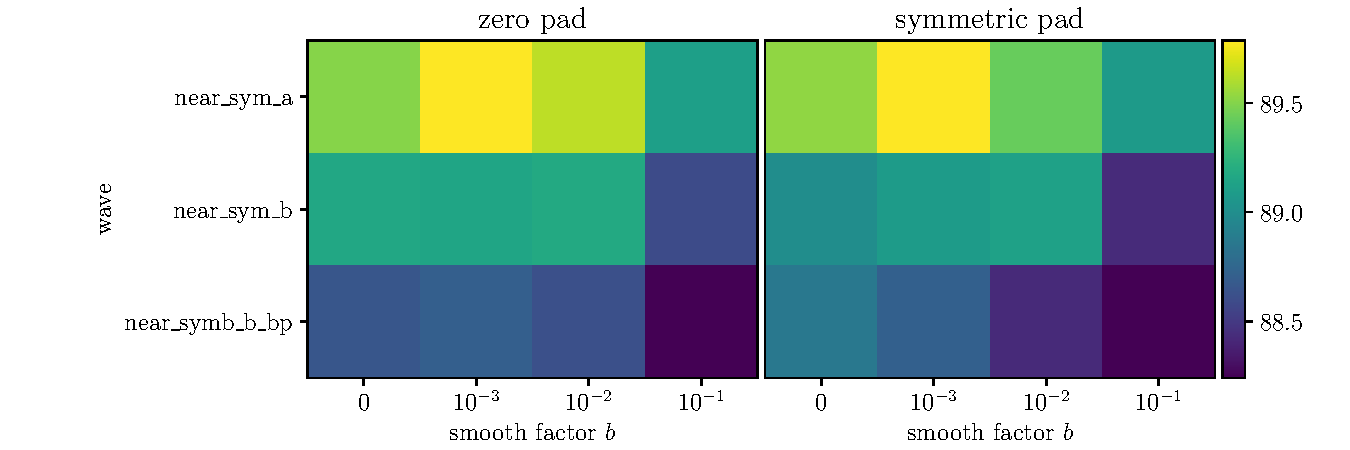
\includegraphics[width=\textwidth]{\imgpath/cifar10_scat_options.pdf}
    \label{fig:ch3:hypes_cifar10}
    }\vspace{-0.3cm}
    \\
  \subfloat[CIFAR-100]{\hspace{-1.2cm}
    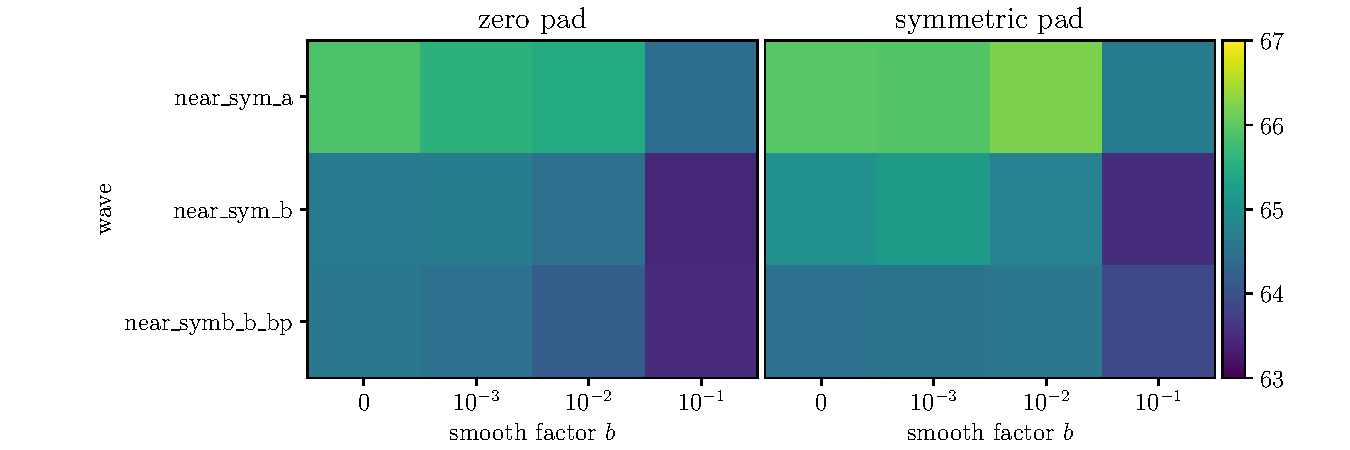
\includegraphics[width=\textwidth]{\imgpath/cifar100_scat_options.pdf}
    \label{fig:ch3:hypes_cifar100}
    }\vspace{-0.3cm}
    \\
  \subfloat[Tiny ImageNet]{\hspace{-1.2cm}
    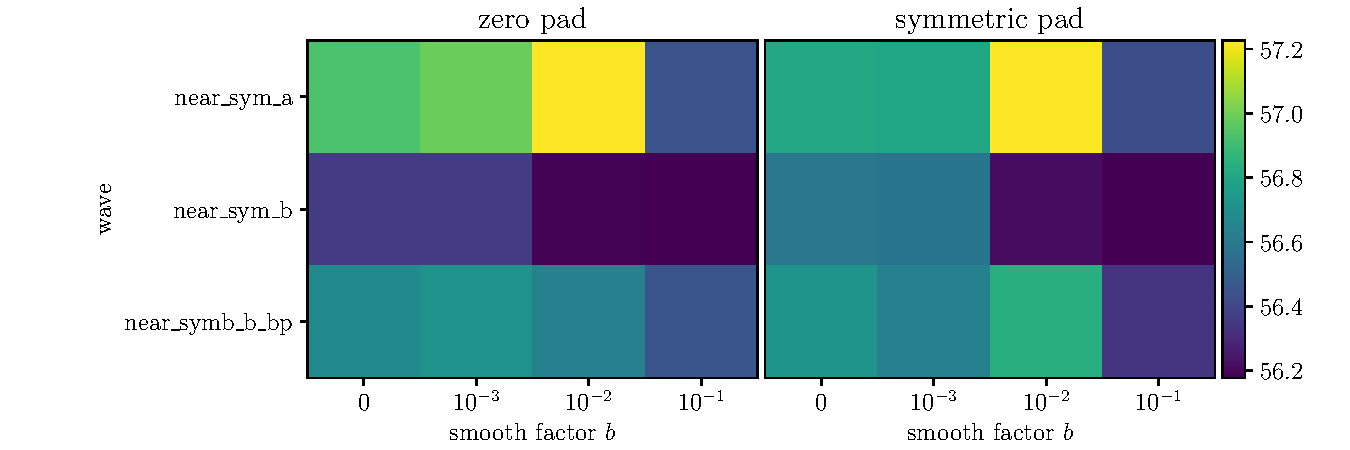
\includegraphics[width=\textwidth]{\imgpath/ti_scat_options.pdf}
    \label{fig:ch3:hypes_ti}
    }\vspace{-0.2cm}
  \mycaption{Hyperparameter results for the $\DTCWT$ scatternet on various
  datasets}{Image showing relative top-1 accuracies (in \%) on the given datasets using
  architecture described in \autoref{tab:ch3:hyper_options}. Each subfigure is a new
  dataset and therefore has a new colour range (shown on the right). Results are
  averaged over 3 runs from different starting positions.
  Surprisingly, the choice of options can have a very large impact on the
  classification accuracy. Symmetric padding is marginally better than zero padding.
  Surprisingly, the shorter filter (near\_sym\_a) fares better than its longer counterparts, 
  and bringing in the diagonal subbands (near\_sym\_b\_bp) does not help.
  Additionally, the smoothing bias may indeed be a good idea for the forward
  pass as well as aiding the backwards pass, so long as it is less than 0.1.}
  \label{fig:ch3:hypes}
\end{figure}

\subsubsection{Results}
We use the optimal hyperparameter choices from the previous section, and compare
these to morlet based ScatterNet with 6 and 8 orientations. The results of this
experiment are shown in \autoref{tab:ch3:comparison}. It is promising to see
that the $\DTCWT$ based scatternet has not only not sped up, but slightly improved
upon the Morlet based ScatterNet as a frontend. Interestingly, both with Morlet
and $\DTCWT$ wavelets, 6 orientations performed better than 8, despite having
fewer parameters in conv1.

\begin{table}[t]
  \centering
  \mycaption{Performance comparison for a $\DTCWT$ based ScatterNet vs
  Morlet based ScatterNet}{We report top-1 classification accuracy for the 3
  listed datasets as well as training time for each model in hours.}
  \label{tab:ch3:comparison}
  \begin{tabular}{lcrrcrrcrr}
    \toprule
    Type & \phantom{abc} & \multicolumn{2}{c}{CIFAR-10} && \multicolumn{2}{c}{CIFAR-100} 
         && \multicolumn{2}{c}{Tiny ImgNet} \\\cmidrule{3-4}\cmidrule{6-7}\cmidrule{9-10}
         && Acc.\ (\%) & Time (h) && Acc.\ (\%) & Time (h) && Acc.\ (\%) & Time (h)\\\midrule
    Morlet8 && 88.6 & 3.4 && 65.3 & 3.4 && 57.6 & 5.6 \\
    Morlet6 && 89.1 & 2.4 && 65.7 & 2.4 && 57.5 & 4.4 \\
    $\DTCWT$ && 89.8 & 1.1 && 66.2 & 1.1 && 57.3 & 2.7 \\\bottomrule
    % \toprule
    % Type & \phantom{abc} & CIFAR-10 & CIFAR-100 & Tiny ImgNet \\ \midrule
    % Morlet8 && & &\\
    % Morlet6 && \\
    % $\DTCWT$ && & 66.2 & 57.2 \\\bottomrule
  \end{tabular}
\end{table}
